\documentclass[aspectratio=169]{beamer}

\usepackage[T2A]{fontenc}
\usepackage[utf8]{inputenc}
\usepackage[english,russian]{babel}
\usepackage{amsmath,amssymb}
\usepackage{graphicx}
\usepackage{microtype}
\usefonttheme[onlymath]{serif}

\usetheme{default}
\setbeamertemplate{navigation symbols}{}

\definecolor{titlered}{RGB}{176,42,42}
\definecolor{slideblue}{RGB}{45,55,140}

\setbeamercolor{structure}{fg=slideblue}
\setbeamercolor{item}{fg=slideblue}

\newlength{\fpmargin}\setlength{\fpmargin}{0.7cm}
\setbeamersize{text margin left=\fpmargin,text margin right=\fpmargin}
\setbeamertemplate{footline}{}

\setbeamertemplate{itemize item}{\color{slideblue}\textbullet}
\setbeamertemplate{itemize subitem}{\color{slideblue!70}--}

\newcommand{\heading}[1]{{\color{slideblue}\bfseries #1}\par\nobreak\smallskip}

\begin{document}

\begin{frame}[plain]
  \vspace{2pt}
  %% ----- только название работы небольшим шрифтом -----
  {\color{titlered}\bfseries\small Применение методов каузального вывода при анализе
    зависимостей между оптимизирующими проходами LLVM-компилятора}

  \vspace{2pt}

  \scriptsize
  \begin{columns}[T]
  %% ===================== ЛЕВАЯ КОЛОНКА: текст =====================
  \begin{column}{0.57\textwidth}

    \heading{Сделали}
    \begin{itemize}\itemsep1pt
      \item Предложен метод оценки \textbf{каузального эффекта} порядка пар
        проходов: случайные перестановки образуют \emph{рандомизированный
        эксперимент} --- эффект оценивается \textbf{без поиска структуры}.
      \item Масштабный эксперимент: \textbf{LLVM~16}, 89~проходов,
        \textbf{517}~программ (LLVM~IR), \textbf{5,17~млн} прогонов (19,3~ч).
      \item Конвейер анализа: ATE по всем $\binom{89}{2}{=}3916$ парам (критерий
        Уэлча, поправка Бенджамини--Хохберга); графы на \textbf{3 уровнях} и
        условный эффект CATE.
    \end{itemize}

    \vspace{1pt}
    \heading{Получили}
    \begin{itemize}\itemsep1pt
      \item Построены \textbf{интерпретируемые каузальные графы} --- основа
        для понимания структуры \textbf{пространства оптимизаций}.
      \item {\color{titlered}\textbf{92,7\,\%}} значимых корреляций
        «порядок\,--\,выигрыш» \textbf{не каузальны}: 608 каузальных рёбер
        против 5124 корреляционных.
      \item \textbf{Валидация}: рёбра \texttt{gvn}$\to$\texttt{instcombine},
        \texttt{gvn}$\to$\texttt{dse} согласуются с реальным \texttt{-Oz}.
      \item Эффект \textbf{гетерогенен}: до \textbf{29\,\%} рёбер меняют знак
        на отдельных типах программ.
    \end{itemize}

  \end{column}
  %% ===================== ПРАВАЯ КОЛОНКА: граф =====================
  \begin{column}{0.42\textwidth}
    \centering
    \heading{\centering Каузальный граф зависимостей}
    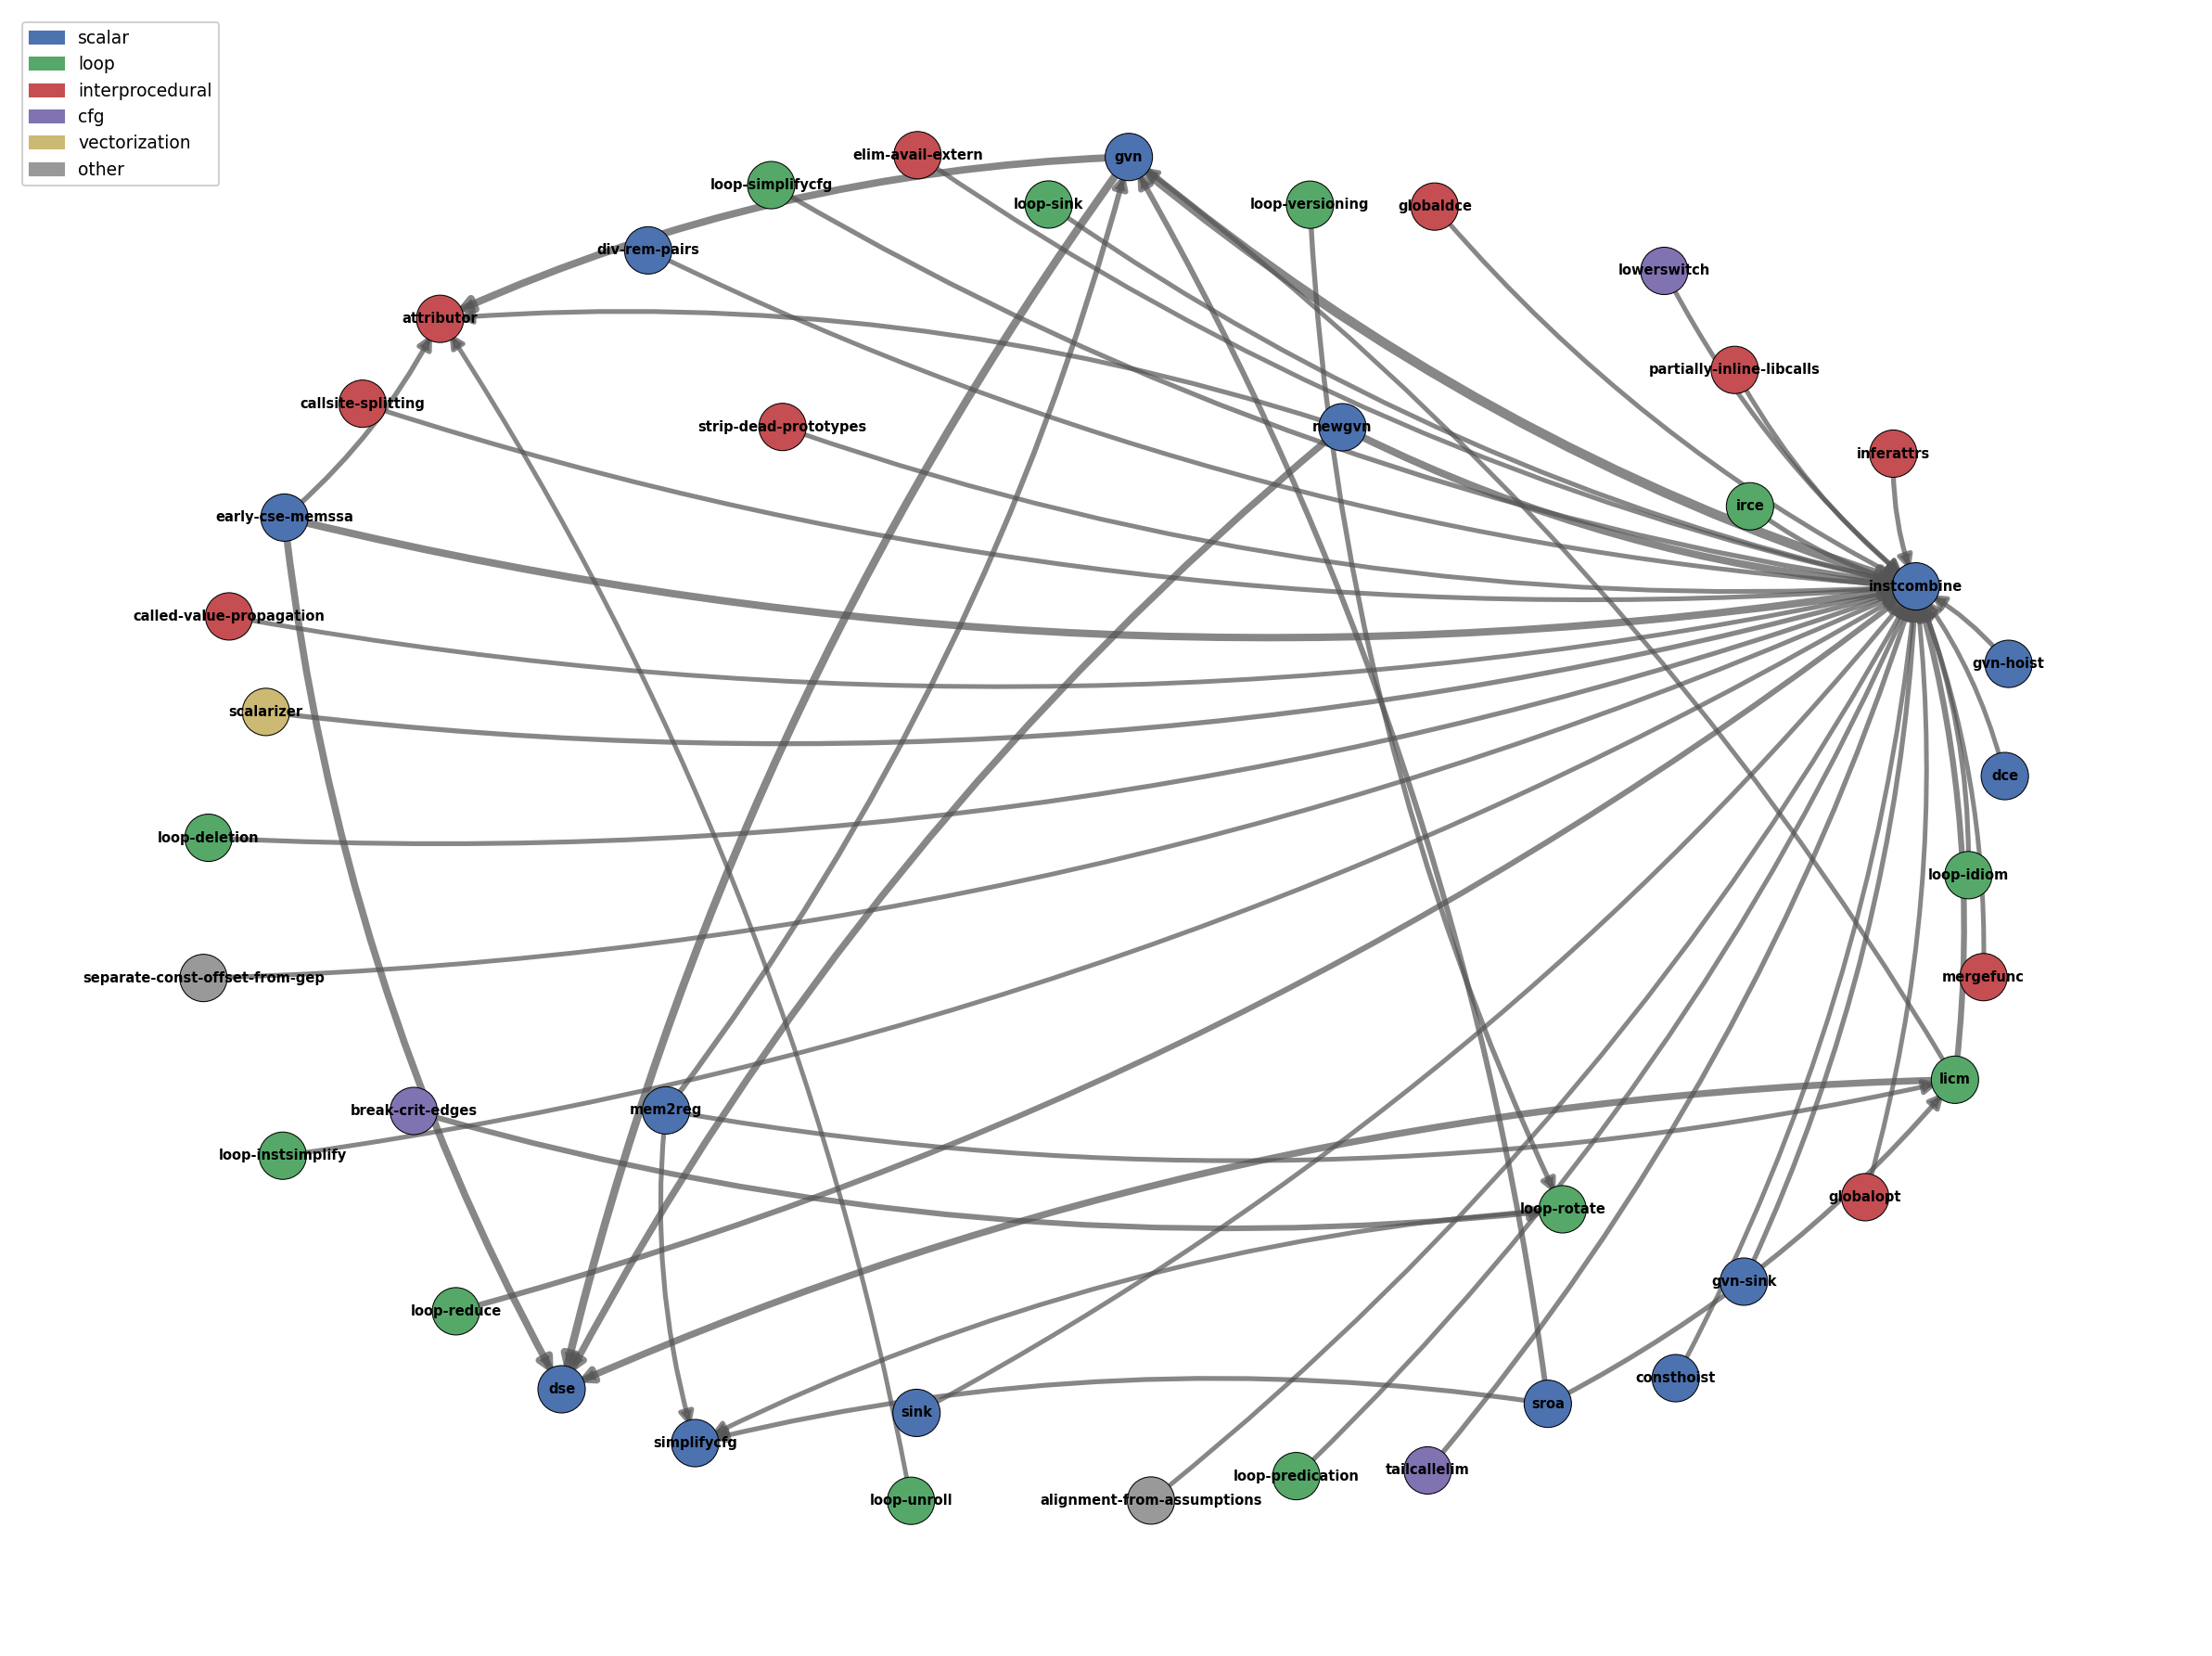
\includegraphics[width=\linewidth]{images/graph_global_top50_filtered.png}\\[1pt]
    {\scriptsize Топ-50 рёбер содержательного графа (372~ребра).\\
      Источники --- проходы нумерации значений (\texttt{gvn}, \texttt{newgvn});
      стоки --- упрощающие (\texttt{instcombine}, \texttt{dse}).}
  \end{column}
  \end{columns}

\end{frame}

\end{document}
